\subsection{Object Selection}

  \paragraph{Accuracy} The Higgs jet selection accuracy is defined as the probability that all four \Pqb-jets in the event are matched to the truth \Pqb-quarks using a $\Delta R$ < 0.3 matching criterion, and is shown is \Fig{\ref{fig:jetSel-4b}}.
  The jet selection accuracy is 74\% for the ggF selection with \%-level variations across the \kl values of interest. 
  This means that there is a \SI{74}{\%} chance the selected four \Pqb-jets are coming from the real Higgs decayed \Pqb-quarks. This accuracy loss is dominated by events where one of the \Pqb-quarks is out of acceptance. 
  The 4b VBF selection has an average \Pqb-quark selection accuracy of 85\% and 90\% for the respective \kl and \kvv signal samples.
  The dependency on \kl and/or \kvv is likely due to the positive dependence of the \Pqb-tagging efficiency on the \Pqb-jet \pt: harder signals lead to higher \Pqb-tagging efficiency therefore higher Higgs jet selection accuracies. 
  \Fig{\ref{fig:jetSel-mhh}} shows the truth \mhh distributions and the reconstructed histograms for the cases where we did or did not selected the correct jets for the ggF and VBF selections at a few signal points. As discussed above, we are less likely to select the correct jets for lower \mhh, and also the signal shapes for the \kl and \kvv variations are quite different, this is entirely due to the underlying \mhh distribution.
    
  \begin{figure}[hbt]
	  \centering
	  \subfloat[Jet selection accuracy vs \kl]{
			   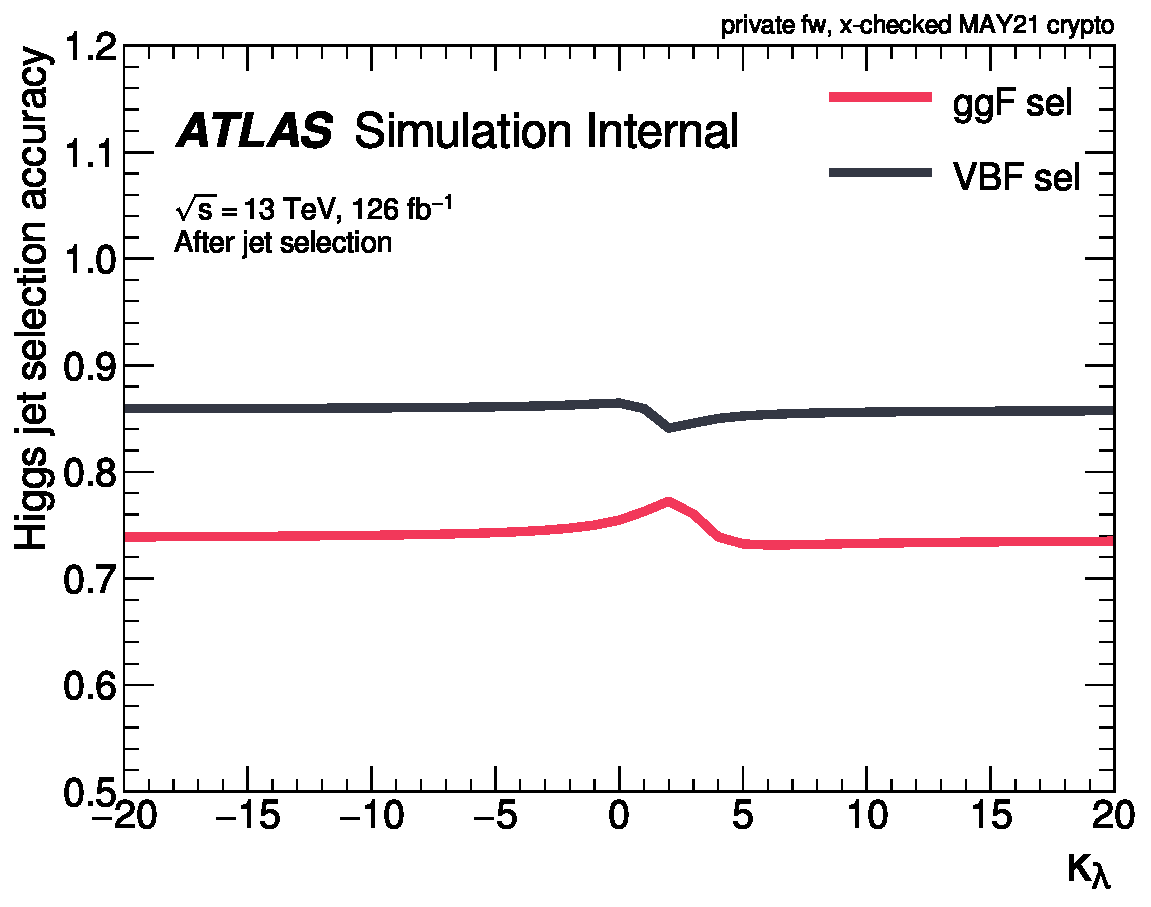
\includegraphics[width=0.4\textwidth]{figures/nr-int-note/selection/V2/jetSel_kl_4b_only.pdf}
		  \label{fig:jetSel-kl}
	  }
	  \subfloat[Jet selection accuracy vs $\kappa_{2V}$]{
			   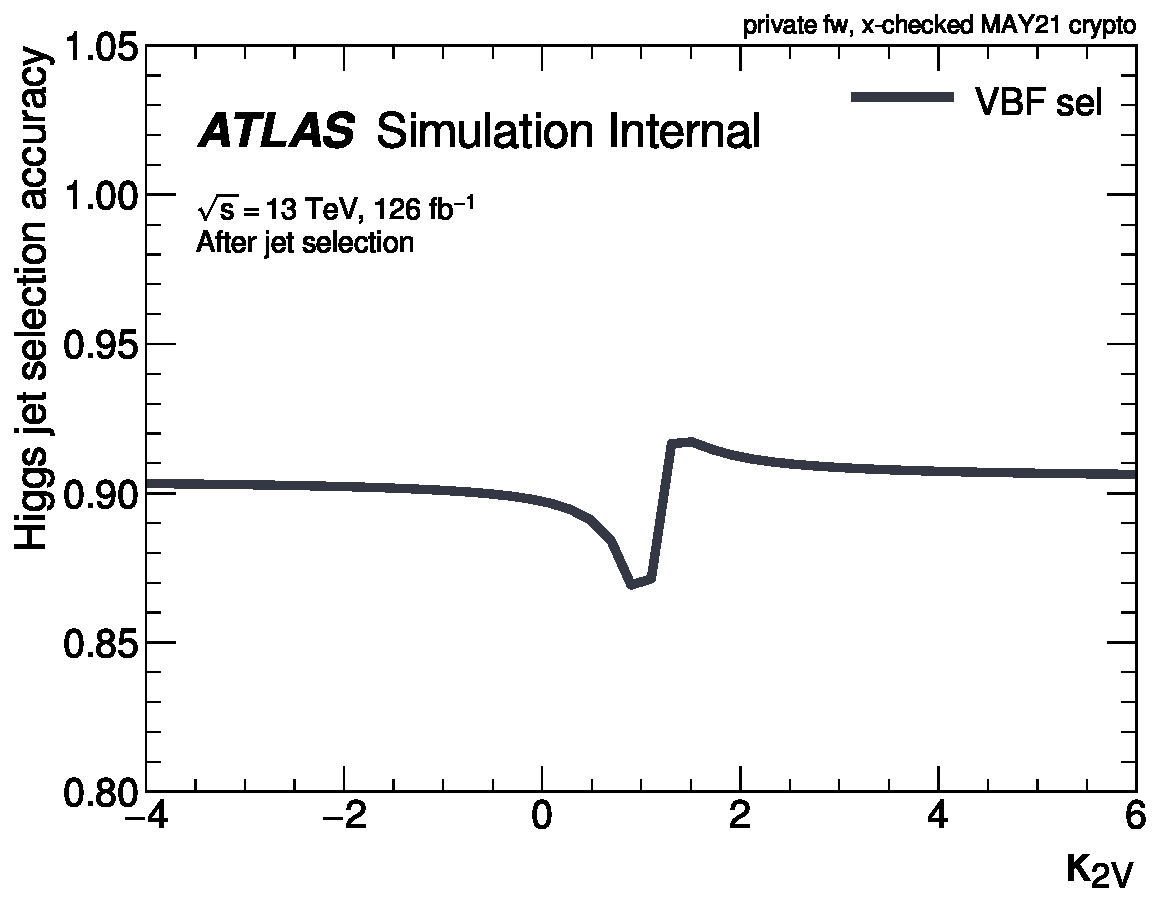
\includegraphics[width=0.4\textwidth]{figures/nr-int-note/selection/V2/jetSel_k2V.pdf} 
		  \label{fig:jetSel-k2V}
	  }
	  \caption{The jet selection accuracy as a function of \kl and \kvv.}
	  \label{fig:jetSel-4b}
  \end{figure}

  \begin{figure}[hbt]
	  \centering
	  \subfloat[ggF signals]{
			   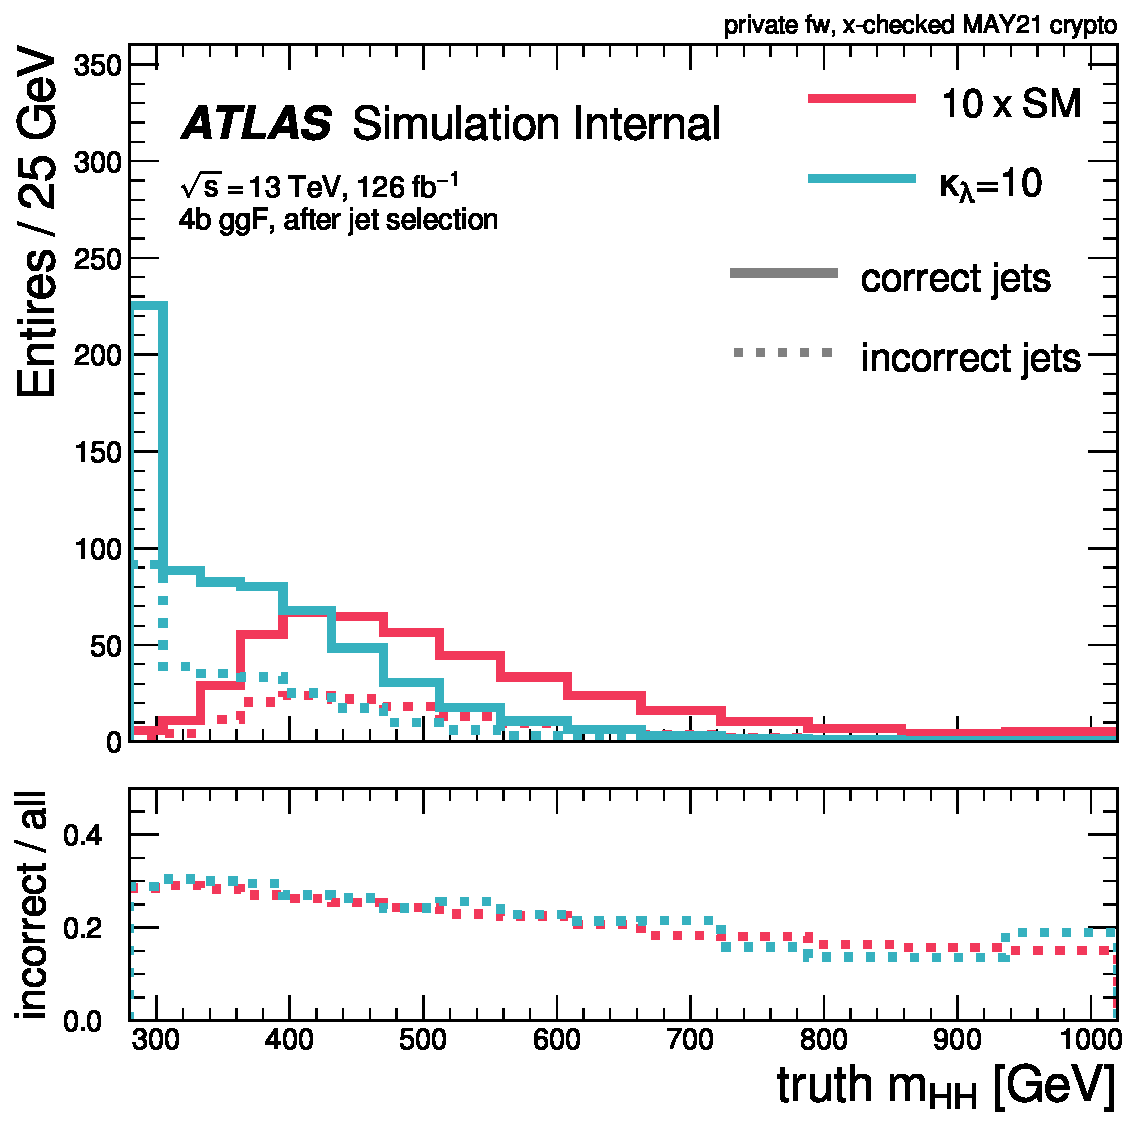
\includegraphics[width=0.4\textwidth]{figures/nr-int-note/selection/V2/truth_mhh_4b_jetSelAcc.pdf}
		  \label{fig:jetSel-kl}
	  }
	  \subfloat[VBF signals]{
			   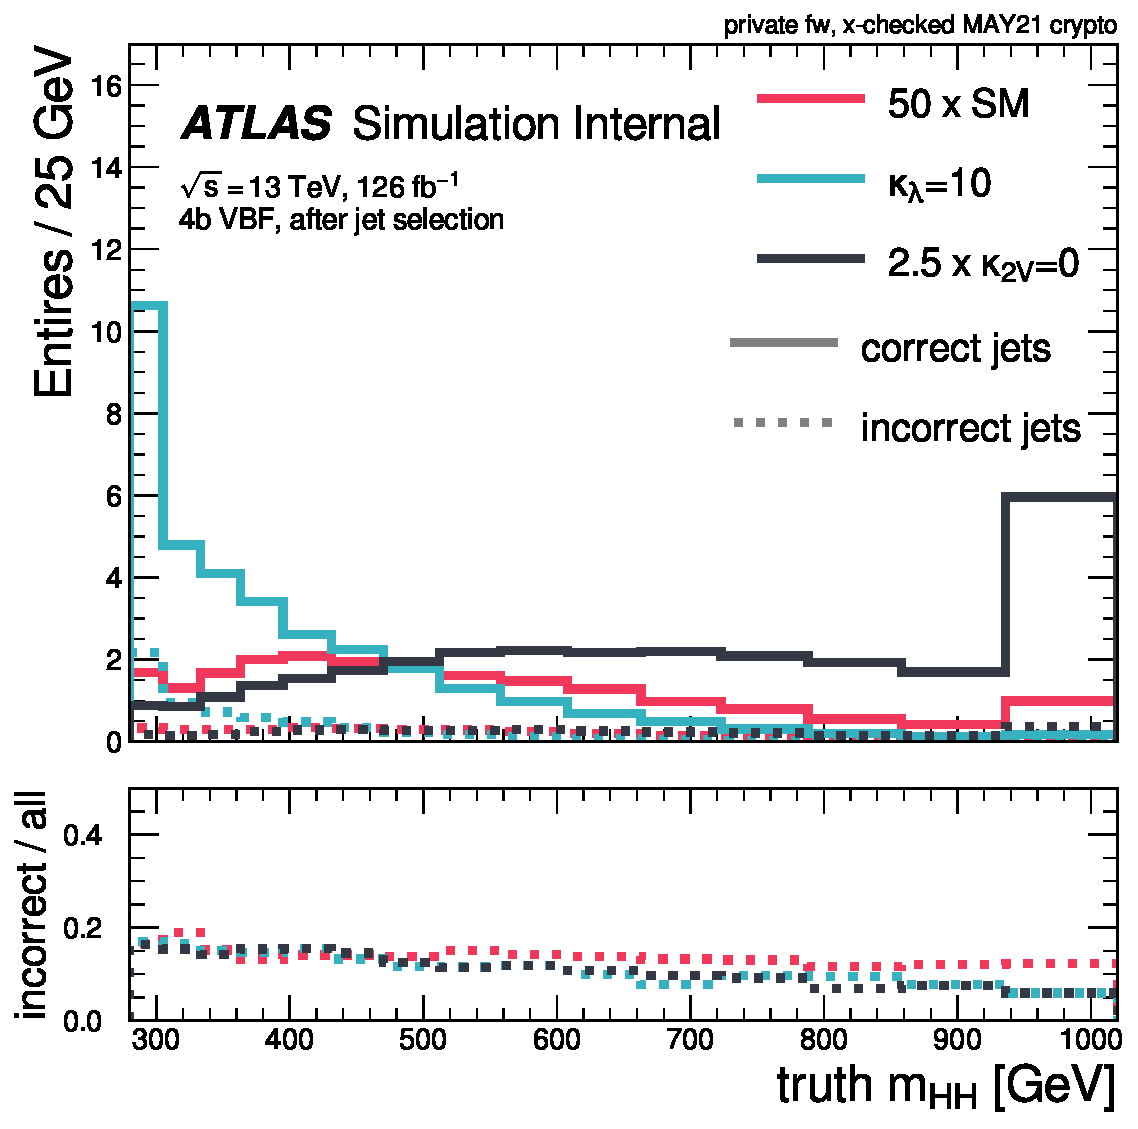
\includegraphics[width=0.4\textwidth]{figures/nr-int-note/selection/V2/truth_mhh_3b1l_jetSelAcc_vbf.pdf} 
		  \label{fig:jetSel-k2V}
	  }
	  \caption{Truth \mhh distributions for correctly and incorrectly selected jets, for ggF (a) and VBF (b) signals.}
	  \label{fig:jetSel-mhh}
  \end{figure}